\documentclass[a4paper,11pt,titlepage]{scrbook}
\usepackage[utf8]{inputenc}
\usepackage[spanish]{babel}

% \usepackage[style=list, number=none]{glossary} %si se va a usar glosario, quitar marca de comentario
%\usepackage{titlesec}
%\usepackage{palatino} %usar fot palatino en vez de times roman

%\decimalpoint %revisar
%\usepackage{dcolumn} %revisat
%\newcolumntype{.}{D{.}{\esperiod}{-1}}
%\makeatletter
%\addto\shorthandsspanish{\let\esperiod\es@period@code}
%\makeatother


%\usepackage[chapter]{algorithm}
%\RequirePackage{verbatim}
%\RequirePackage[Glenn]{fncychap}
\usepackage{fancyhdr}
\usepackage{graphicx}
\usepackage{afterpage}
\usepackage{longtable}
\usepackage{xcolor}
\usepackage{csquotes}
\usepackage{lscape}
\definecolor{portada}{RGB}{239,206,53}
\definecolor{base}{RGB}{35,31,32}
\usepackage{pdfpages}


%Instrucciones para poder escribir código y mostrarlo de manera elegante:
\definecolor{gray97}{gray}{.97}
\definecolor{gray75}{gray}{.75}
\definecolor{gray45}{gray}{.45}
\definecolor{gray30}{gray}{.94}

\usepackage{listings}
\lstset{ frame=Ltb,
framerule=0pt,
aboveskip=0.5cm,
framextopmargin=3pt,
framexbottommargin=3pt,
framexleftmargin=0.4cm,
framesep=0pt,
rulesep=.4pt,
backgroundcolor=\color{gray97},
rulesepcolor=\color{black},
%
stringstyle=\ttfamily,
showstringspaces = false,
basicstyle=\small\ttfamily,
commentstyle=\color{gray45},
keywordstyle=\bfseries,
%
numbers=left,
numbersep=15pt,
numberstyle=\tiny,
numberfirstline = false,
breaklines=true,
literate={á}{{\'a}}1 {Á}{{\'A}}1 {é}{{\'e}}1 {É}{{\'e}}1 {í}{{\'i}}1  {Í}{{\'I}}1  {ó}{{\'o}}1  {Ó}{{\'O}}1  {ú}{{\'u}}1  {Ú}{{\'U}}1  {Ñ}{{\~N}}1 {ñ}{{\~n}}1 ,
}



% minimizar fragmentado de listados
\lstnewenvironment{listing}[1][]
   {\lstset{#1}\pagebreak[0]}{\pagebreak[0]}

\lstdefinestyle{Consola}
   {basicstyle=\scriptsize\bf\ttfamily,
    backgroundcolor=\color{gray30},
    frame=single,
    numbers=none
   }
\lstdefinestyle{C}
	{basicstyle=\scriptsize,
	frame=single,
	language=C,
	numbers=left
	}
\lstdefinestyle{CodigoC++}
        {basicstyle=\small,
	frame=single,
	backgroundcolor=\color{gray30},
	language=C++,
	numbers=left
 	}
\lstdefinestyle{PHP}
	{basicstyle=\scriptsize,
%        {basicstyle=\small,
	frame=single,
	language=PHP,
	numbers=left
	}
	



% ********************************************************************
% Información sobre el TFG. Comentar lo que NO se desee añadir y sustituir con la información correcta.
% ********************************************************************
\newcommand{\myTitle}{NjoyCoking}
\newcommand{\mySubtitle}{Web de geolocalización de recetas}
\newcommand{\myDegree}{Grado en Ingeniería Multimedia}
\newcommand{\myName}{Luis Cobo García}
\newcommand{\myProf}{Pedro Pernías Peco}
\newcommand{\myOtherProf}{Manuel Marco Such}
\newcommand{\myFaculty}{Escuela Politécnica Superior de la Universidad de Alicante}
\newcommand{\myFacultyShort}{EPS UA}
\newcommand{\depTutorOne}{Lenguajes y sistemas informáticos}
\newcommand{\depTutorTwo}{Lenguajes y sistemas informáticos}


\newcommand{\myUni}{\protect{Universidad de Alicante}}
\newcommand{\myLocation}{Alicante}
\newcommand{\myTime}{\today}
%\newcommand{\myVersion}{Version 0.1}

\newcommand{\logoGrado}{imagenes/logoim.jpg}
\newcommand{\logoFacultad}{imagenes/logoeps.jpg}
\newcommand{\logoUniversidad}{imagenes/logoua.jpg}

\usepackage{url}

% Definición de comandos que me son útiles:
%\renewcommand{\indexname}{Índice alfabético}
%\renewcommand{\glossaryname}{Glosario}

\pagestyle{fancy}
\fancyhf{}
\fancyhead[LO]{\leftmark}
\fancyhead[RE]{\rightmark}
\fancyhead[RO,LE]{\textbf{\thepage}}
\renewcommand{\chaptermark}[1]{\markboth{\textbf{#1}}{}}
\renewcommand{\sectionmark}[1]{\markright{\textbf{\thesection. #1}}}


\setlength{\headheight}{1.5\headheight}

\newcommand{\HRule}{\rule{\linewidth}{0.5mm}}
%Definimos los tipos teorema, ejemplo y definición podremos usar estos tipos
%simplemente poniendo \begin{teorema} \end{teorema} ...
\newtheorem{teorema}{Teorema}[chapter]
\newtheorem{ejemplo}{Ejemplo}[chapter]
\newtheorem{definicion}{Definición}[chapter]
 
\newcommand{\bigrule}{\titlerule[0.5mm]}


%Para conseguir que en las páginas en blanco no ponga cabeceras
\makeatletter
\def\clearpage{%
  \ifvmode
    \ifnum \@dbltopnum =\m@ne
      \ifdim \pagetotal <\topskip
        \hbox{}
      \fi
    \fi
  \fi
  \newpage
  \thispagestyle{empty}
  \write\m@ne{}
  \vbox{}
  \penalty -\@Mi
}
\makeatother

\usepackage[pdfborder={000}]{hyperref} %referencia
\hypersetup{
pdfauthor = {\myName (email (en) ua (punto) es)},
pdftitle = {\myTitle},
pdfsubject = {},
pdfkeywords = {palabra_clave1, palabra_clave2, palabra_clave3, ...},
pdfcreator = {LaTeX con el paquete ....},
pdfproducer = {pdflatex}
}
%AQUI COMIENZA LA LISTA DE FICHEROS A INCLUIR

\renewcommand{\baselinestretch}{1.5} %interlineado

\begin{document}
\renewcommand{\listtablename}{Índice de tablas} %para sustituir la palabra cuadro por tabla
\renewcommand{\tablename}{Tabla}
\renewcommand{\lstlistingname}{Listado}
\renewcommand{\lstlistlistingname}{Índice de \lstlistingname s}

\frontmatter
\begin{titlepage}

\newlength{\centeroffset}
\setlength{\centeroffset}{-0.5\oddsidemargin}
\addtolength{\centeroffset}{0.5\evensidemargin}
\thispagestyle{empty}

\includepdf[pages={1},pagecommand={},fitpaper=true,trim=0 0 0 0, 
offset=0 0,turn=true,noautoscale=true]{portada/portada.pdf}

\end{titlepage}
\pagecolor{white} %la portada en color
\begin{titlepage}
 
 
\setlength{\centeroffset}{-0.5\oddsidemargin}
\addtolength{\centeroffset}{0.5\evensidemargin}
\thispagestyle{empty}

\noindent\hspace*{\centeroffset}\begin{minipage}{\textwidth}

\centering


% Title

%{\Huge\bfseries Título del proyecto\\ }
{\Huge\bfseries \myTitle}

\noindent\rule[-1ex]{\textwidth}{3pt}\\[3.5ex]
{\large\bfseries \mySubtitle\\[4cm]}
\end{minipage}

\vspace{2.5cm}
\noindent\hspace*{\centeroffset}\begin{minipage}{\textwidth}
\centering

\textbf{Autor}\\ {\myName}\\[2.5ex]
\textbf{Directores}\\
{\normalsize \myProf\\
\small\textit \depTutorOne\\
\normalsize \myOtherProf\\
\small\textit \depTutorTwo\\[2cm]}

\includegraphics[scale=0.25]{\logoGrado}


\textsc{\myDegree}\\

\centering
\begin{minipage}[l]{7cm}
\includegraphics[width=5cm]{\logoFacultad}
\end{minipage}
\begin{minipage}[r]{7cm}
\includegraphics[width=5cm]{\logoUniversidad}
\end{minipage}


%\textsc{\myFaculty}\\

%\large\bfseries \textsc{\myUni}\\
ALICANTE, \myTime

\end{minipage}
%\addtolength{\textwidth}{\centeroffset}
\vspace{\stretch{2}}

\end{titlepage}


 %la portada en b/n
\chapter*{Preámbulo}





\chapter*{Agradecimientos}

Me gustaría empezar dando las gracias a mi tutor Pedro Pernías. Por sus ideas y consejos que me ha proporcionado durante todo este aprendizaje. Y por su entusiasmo y pasión que me ha transmitido en todas sus clases. Sin él este trabajo no habría cobrado vida.

\vspace{5 mm}

En segundo lugar, agradecer también a mis padres Luis y Raquel, todo el apoyo e interés que me han demostrado durante el desarrollo de este proyecto. Y agradecer todos sus consejos que me han proporcionado durante estos años de carrera.

\vspace{5 mm}

También quiero dar las gracias a la empresa 3dids.com empresa donde he trabajado durante 7 meses, por todo lo que me ha enseñado, ya que sin esos conocimientos no podría haber desarrollado el proyecto con tanta fluidez.


\vspace{5 mm}

Por último agradecer a mi compañero de clase Pablo Pernías, por sus consejos de desarrollo y sugerencias de ampliación y mejora de la aplicación que han servido de gran ayuda para mejorar el proyecto.
 %editar este texto (capitulos/preliminares.tex) para cambiar preámbulo, agradecimientos y dedicatorias
\tableofcontents
\listoffigures
%\listoftables
%\lstlistoflistings

\mainmatter %entre frontmatter y mainmatter, la numeración es en romanos.

%a continuación se propone un esquema de trabajo que puede ser alterado justificadamente.
\chapter{Introducción}


\section{El marketing digital en la web}


\subsection{¿Que és?}

El marketing digital son técnicas y estrategias de comercialización usando medios digitales, tales como dispositivos móviles, televisiores digitales y ordenadores.

\vspace{5 mm}

\textbf{¿Cuáles son las principales diferencias respecto al marketing tradicional?} 

\vspace{5 mm}

\begin{itemize}

\item \textbf{Personalización}: El marketing digital pretende obtener información del usuario más personalizada. Por ello aplica técnicas que permiten que se le sugieran a los internautas información de aquello que está interesado, basado en búsquedas previas o en sus preferencias definidas.

\item \textbf{Masivo}: Se puede obtener un gran número de usuarios que formen parte de tu público objetivo invirtiendo muchos menos dinero que en el marketing tradicional.


\end{itemize}

\subsection{Evolución}

La concepto de marketing digital en la web durante sus inicios hasta la actualidad ha ido ido variando. En los años noventa con la aparición de los primeros banners, aparecen las primeras técnicas de marketing en páginas web aunque este primer concepto que se tiene es mucho más básico y se basaba principalmente en hacer publicidad hacia los usuarios para captar posibles clientes.

\vspace{5 mm}


Con la llegada de las redes sociales y la aparición de los smartphones el concepto de marketing cambia, no se basa únicamente en promocionar un producto. Se pretende crear una estrategia de venta basada en la perspectiva del cliente. Reconociendo e investigando en las áreas que ayuden a los clientes a pensar que sus opiniones importan, genera una fidelidad hacia la marca. Aquí es donde las redes sociales juegan un gran papel, ya que permiten compartir todo tipo de contenido(videos,enlaces,textos) que se asocian a nuestras opiniones y gustos personales. Todo este contenido permite a las empresas conocer más detalladamente a un potencial cliente y así crear estrategías de marketing para fidelizar con él.


\subsection{Técnicas}

Una web es uno de lo mejores sitios para incrementar el prestigio y visibilidad de una marca y alcanzar un mayor rango de clientes con efectividad. Para ello, entran en juego diversas técnicas de marketing digital que nos permiten obtener una mayor visibilidad de marca:

\vspace{5 mm}

\textbf{Posicionamiento SEO}

\vspace{5 mm}

\begin{figure}
\begin{center}
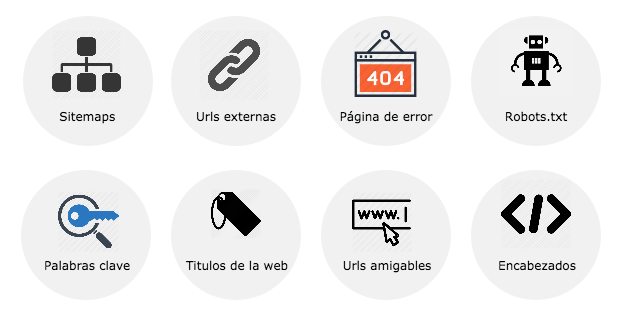
\includegraphics[width=1.0\textwidth]{imagenes/SEO.png}
\caption{Técnicas de SEO}
\label{SEO}
\end{center}
\end{figure}

El posicionamiento en buscadores mejor conocido como posicionamiento SEO es un conjunto de técnicas que implican una mejora de la página web con el fin de mejorar su posición en los resultados de los buscadores para unos términos de búsqueda específicos. Cuanto mejor esta optimizada la página web obtiene una mejor posición en los buscadores y por tanto una mayor visibilidad. En la figura \ref{SEO} se observan las principales técnicas de posicionamiento SEO, que se describen a continuación:

\begin{itemize}

\item \textbf{keywords}: palabras clave, son un conjunto de datos asociados a la página que tienen relación con una posible búsqueda por parte de los usuarios en un buscador. Se asocian como metadatos a una página de la web y son unos de los elementos más básicos para el posicionamiento SEO.

\item \textbf{Urls amigables}: usar palabras cortas y amigables como Urls en el sitio web de vez de urls complejas, permite al buscador disponer de palabras clave para interpretar su contenido. Además es mucho más fácil de interpretar por las personas.

\item \textbf{Etiquetas de Título}: cada página del sitio web, tiene unos metadatos asociados. Una de las etiquetas es el title(título), que indica el nombre de la página web. Es importante que cada página de la web tenga un título diferente y que el texto tenga una información relacionada con la página para facilitar la indexación por parte de los buscadores.

\item \textbf{Mapa de contenido del sitio}: conocido como sitemaps(en inglés), es una lista de las páginas del sitio con información adicional tal como la importancia de la página o la frecuencia con la que cambia de contenidos. Generalmente los sitemaps se generan como fichero XML.

\item \textbf{Página de error personalizada}: una página de error amigable y personalizada mejora la experiencia para el usuario y evita problemas de indexación por parte de los buscadores.

\item \textbf{Insertar links externos}: tener enlaces de otras páginas respetables por los buscadores favorece también a tu sitio al buen posicionamiento.

\item \textbf{Fichero robots}: fichero txt que sirve de guía para los buscadores sobre que información de el sitio web rastrear para posicionarla. Mediante este fichero se delimitan que páginas no queremos que aparezcan posicionadas(página de admin o de política de privacidad por ejemplo) y facilitando la lectura de los crawlers(rastreadores) en el sitio.

\item \textbf{Encabezados de la página}: Utilizar las etiquetas de encabezado(h1,h2,h3) correctamente estableciendo una jerarquía en tu web y utilizados como palabras clave.  


\end{itemize}

\vspace{5 mm}

\textbf{La analítica web}

\vspace{5 mm}

La analítica web nos permite estudiar la repercusión de las campañas de marketing online. Con esta técnica se pretende entender el tráfico del sitio web y así implementar nuevas mejoras en la web.

\vspace{5 mm}

En los inicios de la analítica, el objetivo principal se basaba en medir el número de visitas de un portal web, cuantas más visitas una mayor probabilidad de generar publicidad. En la actualidad se siguen analizando el numero de visitas de un sitio, pero la analítica web sigue evolucionando y se empiezan a medir otros indicadores como la profundidad de las visitas. Las métricas mas importantes utilizadas se dividen en dos tipos, básicas y avanzadas.


\textbf{Métricas básicas}: Nos permiten ver el tráfico en la web: 

\begin{itemize}

\item \textbf{Visitas}: Número de visitas de la página.

\item \textbf{Tasa de rebote}: Mide el número de personas que llegan a una determinada página del sitio.

\item \textbf{Tasa de salida}: Conocer las páginas de la web en las que los visitantes abandonan la web.

\item \textbf{Fuentes de tráfico}: Analiza las fuentes de donde provienen las visitas de los usuarios. 

\end{itemize}

\vspace{5 mm}

 \textbf{Métricas avanzadas(KPI)}: indicadores clave del rendimiento del sitio web. Estás metricas se basan en la comparación de los objetivos marcados por la empresa a lo conseguido. En función del tipo del sitio web los KPIs serán diferentes:

\begin{itemize}

\item \textbf{Sitio web de contenido}: para un sitio web de contenidos los objetivos principales son captar tráfico y fidelizar con el usuario de forma que vuelva otra vez al sitio web. Para este sitio se emplearían KPIs tales como:

- La profundidad de las visitas. Tasa que mide la cantidad de páginas de la web que ve un usuario en una visita.

- Tasa de conversion. Porcentaje que se obtiene del número de conversiones entre el número de visitas. Las conversiones. La definición de conversión dependerá del tipo de web. Para un sitio con contenidos las conversiones equivalen al número de registros en la aplicación.

\item \textbf{Sitio web de ventas}: El objetivo principal de una tienda online es conseguir el mayor número de ventas. Para ello  se utilizarían los siguientes KPIs:

- Ingresos por visita. Porcentaje que expresa el número de ingreso de la tienda en función del número de visitas a la web.

- Cantidad media por pedido. Esta tasa mide la cantidad total de ingresos obtenidos por la empresa entre el número de ventas realizadas.

\end{itemize}

\begin{figure}
\begin{center}
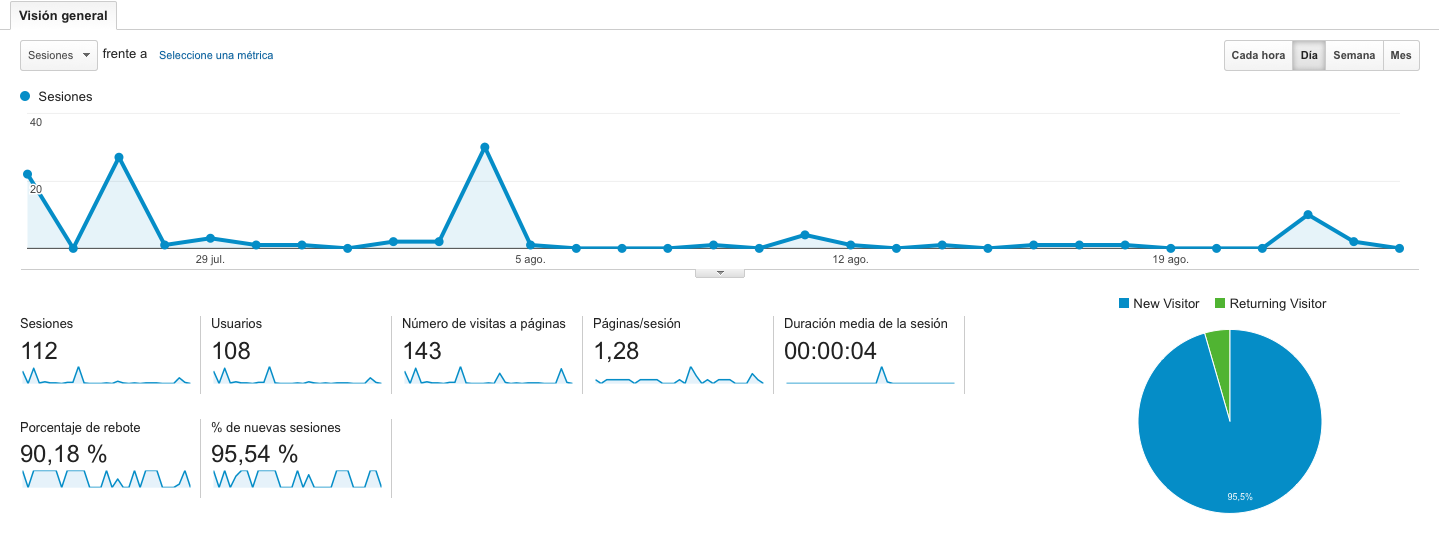
\includegraphics[width=1.0\textwidth]{imagenes/analytics.png}
\caption{Panel de analytics}
\label{analytics}
\end{center}
\end{figure}

Para monitorizar toda el tráfico de datos obtenido de las métricas aplicadas se usan herramientas de analítica web. Una excelente herramienta gratis es Google Analytics, que proporciona un dashboard muy completo para monitorizar la información de tu sitio web.

\textbf{La redes sociales} 

\vspace{5 mm}

Con la aparición de las redes sociales y su gran apogeo entre los usuarios de internet, las empresas ven una herramienta muy potente para promover sus marcas. Las principales técnicas de social media marketing, adaptadas a las necesidades de cada empresa  puede reportar muchos beneficios:

\begin{itemize}

\item \textbf{Difusión}: se consigue una difusión de la información rápida y económica.

\item \textbf{Recopilación de datos}: Se obtiene una gran cantidad de información(BIG DATA) sobre el público objetivo de la marca utilizando una táctica para las redes sociales.

\item \textbf{Mayor número de visitas}: Mediante la difusión de contenido en redes sociales y con una buena táctica bien orientada se consigue una mayor visibilidad de tu sitio web.

\end{itemize}

Como se dice previamente, del uso de tácticas de social media, se obtiene una recopilación de datos relevante para ser utilizados por una empresa con el fin de afianzar la fidelidad con sus clientes o conseguir nuevos. Con los datos obtenidos de las redes sociales las empresas pueden analizar la información y utilizarla sabiamente para dar una mayor visibilidad a su marca. Un ejemplo de uso de los datos de redes sociales podría ser la obtención de un nicho de mercado sobre el que la empresa pueda generar un nuevo modelo de negocio.


\subsection{El caso de Twitter}
\chapter{Marco Teórico}
\label{marcoteorico}

%Aquí va una lista:
%\begin{itemize}
    %\item Ingeniería Informática.
    %\item Ingeniería Sonido e Imagen en Telecomunicación.
    %\item Ingeniería Multimedia.
    %\begin{itemize}
         %\item Mención: Creación y ocio digital.
         %\item Mención: Gestión de Contenidos.
    %\end{itemize}
%\end{itemize}




\begin{figure}
\begin{center}
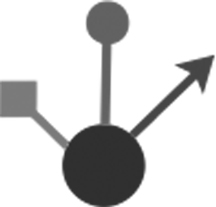
\includegraphics[scale=0.25]{imagenes/logoim.jpg}
\caption{Logo de Ingeniería  Multimedia.}
\label{logo_im}
\end{center}
\end{figure}

\begin{figure}
\begin{center}

\includegraphics[scale=0.25]{imagenes/logoeps.jpg}
\caption{Logo de la EPS.}
\label{logo_eps}
\end{center}
\end{figure}

\section{El marketing digital en la web}

 \cite{listing_packagge} y en \cite{heinz1listings}.

Otro ejemplo, ahora para mostrar código PHP, sería escribir en tu fichero \LaTeX lo siguiente:
\begin{verbatim}
 \begin{lstlisting}[style=PHP, caption={ejemplo código PHP},label=PHP_code]
 /* 
Ejemplo de código en PHP para escribir tu primer programa en este lenguaje
Copia este código en tu ordenador y ejecútalo
*/
<html>
  <head>
    <title>Prueba de PHP</title>
  </head>
  <body>
    <?php echo '<p>Hola Mundo</p>'; ?> //esto lo escribe TODO el mundo
  </body>
</html>
 \end{lstlisting}
\end{verbatim}
 
 y el resultado es: (ver listado \ref{PHP_code})
 
\chapter{Objetivos}


\section{Objetivo Principal}

\displayquote{``Desarrollar una herramienta que permita conocer, según localización geográfica, lo que los usuarios están publicando en distintas redes sociales acerca de temas culinarios orientada para su uso en el marketing y promoción de un portal de cocina.''}

Ello permitirá enfocar mejor las campañas de difusión y promoción de productos de ese sector a un público concreto al localizarlo geográficamente.

\vspace{5 mm}

\section{Objetivos Específicos}

\begin{itemize}
  \item Definir los requisitos y espicificaciones de la aplicación.
  \item Estudiar de las diversas API's a utilizar en el proyecto y conocer su uso.
  \item Diseñar una arquitectura de software capaz de recoger información de las diferentes redes sociales y almacenarla de forma eficaz en la base de datos.
  \item \textbf{Testear y Probar} la aplicación en diferentes navegadores y dispositivos.
  \item Proporcionar un \textbf{producto minimo viable(PMV)} de la aplicación y un modelo de negocio basado en el.
\end{itemize}



\chapter{Metodología}

Para la realización de este proyecto, se estimó una duración de 5 meses donde 1 mes se dedicaría a la investigación, 1 mes para la especificación y diseño y 3 meses para el desarrollo. 

\vspace{5 mm}

Para elegir el marco de trabajo a usar en el desarrollo se tienen en cuenta algunas de las características de las aplicaciones web:

\begin{itemize}

\item La habilidad para manejar el crecimiento continuo del trabajo de manera fluida(Escalabilidad).  

\item La facilidad para comunicarse con diferentes protocolos e interfaces de datos(Interoperabilidad). 

\item La habilidad para medir el correcto funcionamiento del sistema y sus componentes mediante pruebas(Capacidad de Prueba). 

\end{itemize}


\vspace{5 mm}

Con esas características y sabiendo que el desarrollo del sistema se creará de forma iterativa, se opta por utilizar una metodología ágil. Despues de estudiar detalladamente cada una de las metodologías ágiles, finalmente se optó por usar Scrum \cite{scrum}.

\vspace{5 mm}

La metodología Scrum se basa en la realización de pequeños sprints(periodos en el cual se lleva a cabo el trabajo) de 2 o 3 semanas. Al inicio de cada sprint se lleva a cabo una reunión de planificación donde se especifica el trabajo que se va a realizar y se estiman el tiempo en horas que se va a tardar. Cuando finalize el sprint se realizará una revisión comprobando que se ha completado el trabajo.

\vspace{5 mm}

Ventajas de trabajar con la metodología SCRUM:

\begin{itemize}

\item Reducción de riesgos. Como el alcance está limitado al entregable del sprint comprometido, la aparición de riesgos se limita únicamente a lo que se va a desarrollar.

\item Se pueden priorizar los requisitos de la aplicación por valor y coste. En función al valor que aportan que aportan a la aplicación y el coste que supone desarrollarlas se priorizan para proporcionar el resultado más óptimo en el proyecto. Esta lista de requisitos priorizada se denomina Product Backlog.

\item Flexibilidad y adaptación. Al final de cada sprint se puede aprovechar la parte completada para hacer pruebas y sobre el resultado obtenido tomar decisiones.

\item Productividad y calidad. SCRUM se sirve de un proceso de mejora continua, comunicación diaria entre las partes implicadas, estimaciones de esfuerzos conjuntas y entrega de productos de forma regular. Todo ello, con la consigna de mejorar y simplificar la iteración anterior.

\end{itemize}
%!TEX root = .../tfg_im.tex

\chapter{Desarrollo}

\section{Descripción}

\subsection{Funciones del sistema}

La aplicación que se va a desarrollar tiene como objetivo recoger información de las diferentes redes sociales, almacenarlos en una base de datos y
mostrarlos en nuestro sitio web. Esos datos almacenados,serán una fuente de información fiable que permitirá conocer que se esta concinando en el mundo
en este momento. Para ello se deberá tener en cuenta la gestión de:

\begin{itemize}

\item \textbf{Gestión de Usuarios}. En la aplicación, se podrán dar de alta usuarios. Existirán tres tipos de roles de usuario:

\begin{itemize}
\item \textbf{Administrador}. Tendrá el control de gestionar la información proveniente de las API's.El Filtrado de los datos o la frecuencia con la que realiza las peticiones la aplicación con las API's.
También podrá gestionar el contenido del sistema
\item \textbf{Colaborador}. Podrá publicar contenido en la aplicación.
\item \textbf{Usuario no registrado}. Tendrá acceso a la visualización de los datos de la aplicación.
\end{itemize}

\item \textbf{Obtención de datos}. Se podrá consultar información en detalle sobre un elemento de la web.

\item \textbf{Búsqueda}. Existirán varios métodos que permitirán al usuario filtrar la información deseada.

\end{itemize}

\section{Análisis}

Para el desarrollo de la aplicación se lleva a cabo previamente un análisis de las diferentes herramientas utilizadas.

\subsection{Twitter}

Twitter es la red social de \textquote{microblogging} más conocida actualmente. Esta red social tiene más de 500 millones de usuarios, generando un número aproximado de 65 millones de tweets al dia.
Es por ello que se optó por Twitter, ya que es una gran fuente de información en tiempo real.

\vspace{5 mm}

Toda la información proveniente de Twitter es guardada en la base de datos de la aplicación. Para obtener la información,
Twitter habilita una REST API que proporciona a los desarrolladores un acceso a la lectura y escritura de gran parte de la información disponible
en la red social \cite{twitter-api}.

\vspace{5 mm}

\textbf{Twitter API}

\vspace{5 mm}

\begin{landscape}
\begin{figure}
\begin{center}
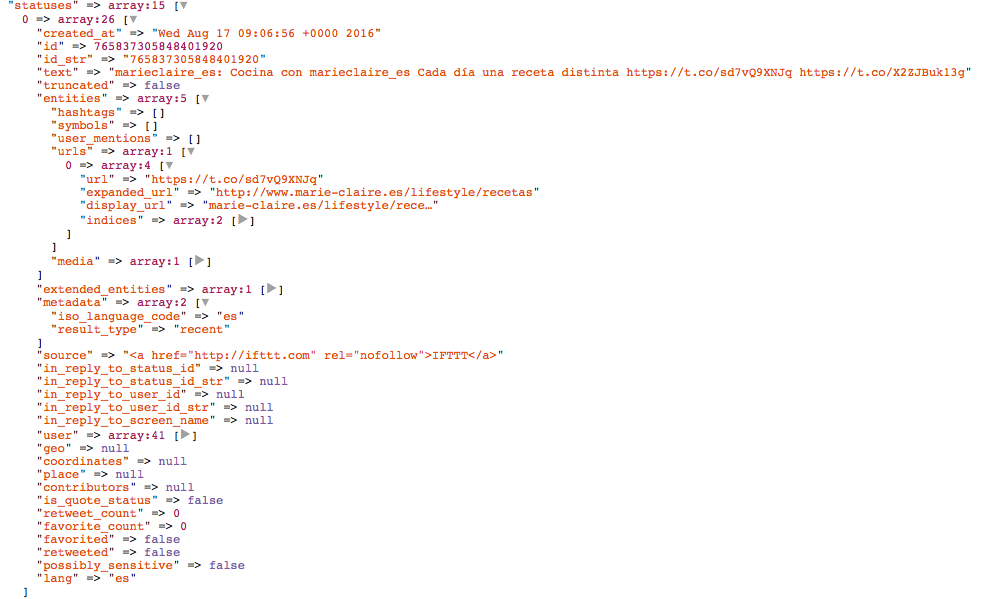
\includegraphics[width=16cm]{imagenes/estructura-tweet.png}
\caption{Un tweet}
\label{tweet}
\end{center}
\end{figure}
\end{landscape}

La REST API de Twitter nos proporciona los datos en formato JSON listos para ser procesados. Un Tweet, contiene una estructura(ver figura \ref{tweet}) elaborada con toda la información relacionada. La estructura de un Tweet consta de los siguientes elementos:

\begin{itemize}

\item \textbf{created\_at}. Fecha de creación del Tweet, contiene el día, mes, hora, zona horaria y año de cuando se ha creado el Tweet.
\item \textbf{id}. Identificador único del Tweet
\item \textbf{id\_str}. El identificador del Tweet en formato de cadena de texto. Este campo esta creado para ciertos lenguajes que no soportan enteros mayores de 53 bits, como es el caso de Javascript.
\item \textbf{text}. Contiene la información del Tweet(máximo de 140 caracteres).
\item \textbf{truncated}. Booleano que especifíca si el valor del campo text está cortado. El texto truncado terminará con los tres puntos suspensivos.
\item \textbf{entities}: Proporciona metadatos asociados al contenido del tweet. Entities es un objeto que contiene los siguientes elementos:

\begin{itemize}

\item \textbf{hashtags}. Representa un array con los hashtags parseados en el contenido del tweet. Cada hastag contiene un campo de texto con el contenido del hashtag y un array de enteros indicando la posicion inicial y final que ocupa en el Tweet.

\item \textbf{media}. Array de objetos que representa el contenido multimedia subido en el Tweet. Este array contiene la url para mostrar a los clientes(display\_url). Una versión expandida de la url(expanded\_url). El id del fichero y el id en formato de cadena de texto(id\_str). Un array con los indíces de la posiciones inicial y final de la url en el texto. Una url apuntando directamente al fichero subido(media\_url) y una url para páginas https(media\_url\_https). Un objeto con los tamaños disponibles para el fichero(sizes).Para aquellos tweets que tiene contenido multimedia asociado a otros tweets, se guarda un identificador que apunta al Tweet con el contenido original(source\_status\_id). El tipo de fichero(type) y la url incrustada en el contenido del Tweet(url).

\item  \textbf{url}. Contiene un array de objetos que representan las urls incluidas en el texto. Contiene la url de visualización, la url expandida y los indices donde se encuentra la url.

\item \textbf{user\_mentions}. Representa otros usuarios de twitter mencionados en el texto del tweet. Este array tiene el id del usuario mencionado, el id en string, los indices y el nombre(name).

\end{itemize}


\item \textbf{metadata}. Array de objetos metadatos asociados al tweet.

\begin{itemize}

\item \textbf{iso\_language\_code}. Codificación iso del lenguaje del tweet.

\item \textbf{result\_type}. Especifica el tipo de resultado de tweet que quieres recibir. El valor por defecto es recent que devuelve un resultado con los tweets más recientes. También están los valores popular que devuelve los tweets más populares y mixed que incluye ambos tipos mencionados anteriormente.

\end{itemize}


\item \textbf{in\_reply\_to\_status\_id}. Si el tweet es una respuesta de otro tweet, este campo tendrá el id del tweet orginal.

\item \textbf{in\_reply\_to\_user\_id}. Contendrá el id del usuario del Tweet original.

\item \textbf{user}. Contiene un array de objetos con toda la información relativa a el usuario que ha publicado el Tweet.

\begin{itemize}

\item \textbf{id}. id del usuario que pública el Tweet.

\item \textbf{name}. Nombre del usuario.

\item \textbf{location}. Cadena de caracteres con el sitio geaográfico al que pertenece el usuario.

\item \textbf{description}. Pequeño resumen descriptivo sobre el usuario.

\item \textbf{url}. Url proporcionada por el usuario asociada con su perfil.

\item \textbf{followers\_count}. Número de seguidores que tiene el usuario.

\item \textbf{friends\_count}. Número de personas a las que sigue el usuario.

\item \textbf{protected}. Indica si la cuenta del usuario esta protegida, es decir que sus Tweets solo pueden ser vistos con el consentimiento del usuario.

\item \textbf{geo\_enabled}. Indica si el usuario a activado la posibilidad de geoetiquetar sus Tweets, es decir, agregar información geográfica en los metadatos del tweet.


\end{itemize}

\item \textbf{coordinates}. Representa la posicion geográfica del Tweet. El array de coordenadas esta en geoJSON, donde la longitud es el primer elemento del array y la latitud el segundo.

\item \textbf{place}. Cuando el Tweet esta asociado a un lugar, pero no necesariamente es orginado de ahí.

\item \textbf{retweet\_count}. Numero de veces que el Tweet ha sido retweeteado.

\item \textbf{lang}. Idioma en el que esta escrito el Tweet.

\end{itemize}

\vspace{5 mm}

Con el análisis de la estructura de un Tweet realizado, se procede a buscar información en Twitter sobre datos relevantes para la aplicación.
Para encontrar los datos relevantes que se ajusten a los requisitos para la aplicación, la API de Twitter proporciona unas opciones de búsqueda que
permiten buscar los Tweets por palabras clave, idioma, localización y número.

\vspace{5 mm}

Para el caso de Njoycooking, se pretendía inicialmente buscar Tweets en español de la zona de la península Ibérica que tuvieran la palabra receta, cocina o comida en el Tweet. Para ello utilizaremos los siguientes parametros que Twitter proporciona:

\begin{itemize}

\item \textbf{q}: parámetro para realizar un consulta de búsqueda por palabras.

\item \textbf{geocode}: parámetro que permite encontrar Tweets de usuarios localizados en un radio alrededor de un punto central proporcionado en latitud/longitud. Por ejemplo para buscar Tweets de la peninsula establecemos el centro en Madrid que en coordenadas lat/long es (39.8952506,-3.46863775058), y le decimos el radio de alcance, aproximadamente unos  500km.

\item \textbf{lang}: parámetro que restringe la búsqueda de Tweets al idioma dado. Si solo utilizaramos el parámetro geocode twitter también nos sacaría resultados de Tweets en portugues, para ello se añade este parámetro indicandole que busque por el idioma español(es).

\item \textbf{count}: parámetro que sirve para definir el número de Tweets a devolver por consulta. Por defecto son 15 y se puede buscar hasta un máximo de 100.


\item \textbf{until}: devuelve los Tweets creados antes de la fecha dada. Este parámetro no tiene mucho sentido que se utilize, ya que lo que se pretende es buscar los últimos Tweets en tiempo real y no buscar por una fecha determinada.

\item \textbf{result\_type}: parámetro para especificar el tipo de resultado de búsqueda. Los tipos son mixed,recent,popular. Para la aplicación interesa el tipo de resultados recent, ya que nos devuelve los Tweets más recientes.

\end{itemize}


\subsection{Google Maps}

 En la actualidad, con el auge de los dispositivos móviles, cada vez es más fácil encontrar el restaurante deseado o la tienda preferida con
 una sola búsqueda en nuestro smartphone. A los negocios locales les interesa tener visibilidad en internet para poder darse a conocer con facilidad y tener un mayor número de clientes. Aquí es donde entra en juego Google Maps, herramienta que permite representar de manera precisa en un mapa un negocio, punto de interés o edificio emblemático de una ciudad.

\vspace{5 mm}

Google maps es una de las herramientas más potentes actuales para la geolocalización y por tanto es la más utilizada. Porporciona un API que te permite incluir un mapa en tu sitio web, personalizar iconos y estilos del mapa y además manejar los eventos \cite{googleMaps-api}. La estructura de la API de Maps es la siguiente:

\vspace{5 mm}

\textbf{Eventos}

\vspace{5 mm}

 \textbf{Eventos de usuario}: Sirven para controlar las acciones que realizan los usuarios y especificar como se va a comportar la página ante ellos. Algunos de los eventos de usuario disponibles en la API de maps son los siguientes:

\begin{itemize}

\item click: Click izquierdo sobre el elemento.

\item rightclick: Click derecho sobre el elemento.

\item dbclick: Doble click sobre el elemento.

\item drag: Arrastrar sobre el elemento.

\item mouseover: El ratón está sobre el elemento que tiene el evento.

\item mouseout: El ratón esta fuera del elemento que tiene el evento.

\end{itemize}

\textbf{Eventos de cambios de estado}: Sirven para controlar las modificaciones de las propiedades de los objetos de la API. Se pueden interceptar estos eventos mediante el controlador addListener().

\vspace{5 mm}

\textbf{Tipos de Mapa}

\vspace{5 mm}

Existen cuatro tipos de mapas básicos disponibles en la API de Google Maps. Los mapas básicos son:

\begin{itemize}

\item MapTypeId.ROADMAP. Vista del mapa de carreteras. Predeterminado.

\item MapTypeId.SATELLITE. Imágenes del satélite de Google Earth.

\item MapTypeId.HYBRID. Combina las vistas de satélite y del mapa de carreteras.

\item MapTypeId.TERRAIN. Mapa basado en información terrestre.

\end{itemize}

\vspace{5 mm}

Para personalizar los mapas básicos la API te permite cambiar la visualización de elementos como carreteras, áreas de edificios y parques utiliando estilos. Cada elemento del mapa se especifica mediante el tipo MapTypeStyleFeatureType. Las funciones se especifican con la sintaxis featureType: 'característica'. Las características disponibles son:

\begin{itemize}

\item road: selecciona las carreteras(autovías,locales).

\item landscape: selecciona los elementos naturales(bosques,terrenos).

\item poi: selecciona los puntos de interés(negocios,ayuntamientos,parques).

\item administrative: selecciona las áreas administrativas(países,províncias,localidades,etc).

\item transit: selecciona toda las estaciones de tránsito de transportes públicos(autobús,aeropuerto,etc).

\item water: selecciona las zonas de agua(mares, lagos, ríos).

\end{itemize}

\vspace{5 mm}

Cada una de las funciones de características del mapa se compone de varios elementos. Los tipos de elementos disponibles son:

\begin{itemize}

\item all: selecciona todos los elementos de la función.

\item geometry: selecciona todos los elementos geométricos.

\begin{itemize}

\item geometry.fill: selecciona el relleno de la geometría.

\item geometry.stroke: selecciona el trazo de la geometría.


\end{itemize}

\item labels: selecciona las etiquetas de texto asociadas.

\begin{itemize}

\item labels.icon: selecciona únicamente el icono que se muestra dentro de la etiqueta.

\item labels.text: selecciona el texto de la etiqueta.

\item labels.text.fill: selecciona el relleno de la etiqueta.

\item labels.text.stroke: selecciona únicamente el trazo del texto del a etiqueta.

\end{itemize}

\end{itemize}

\vspace{5 mm}

Una vez seleccionado la caracteística y su correspondiente elemento que se quiere personalizar, se aplican los parámetros de estilo que son opciones del tipo MapTypeStyler y son las que modifican la apariencia de la característica. Las opciones de estilo disponibles son:

\begin{itemize}

\item lightness: valor entre -100(negro) y 100(blanco) indica el porcentaje de brillo del elemento.

\item saturation: valor entre -100 y 100 indica el porcentaje de intensidad.

\item visibility: especicifica si el elemento aparece en el mapa(on/off) y la forma en la que aparece(simplified). Mediante la visibilidad simplified se eliminan algunas funciones de estilo del elemento.

\item color: color del elemento(cadena RGB hexadecimal).

\item hue: color básico(cadena RGB hexadecimal).

\item gamma: valor entre 0.01 y 10.0, se usan para modificar el contraste en varios elementos.

\end{itemize}

\vspace{5 mm}

\textbf{Marcadores}

Los marcadores son unos de los elementos más utilizados y relevantes de la API de Google ya que representan una ubicación exacta en un punto del mapa. Los marcadores son objetos del tipo \textquote{Marker} y se incializan mediante el constructor google.maps.Marker. Al construir un marcador un marcador se especifican sus propiedades iniciales:

\begin{itemize}

\item position: Objeto de tipo LatLng(latitud,longitud) que define el punto inicial del marcador.

\item map: Mapa donde debe representarse el marcador.

\end{itemize}

Para mostrar contenido en el mapa la API proporciona los objeto InfoWindow que muestran la información en una ventana emergente. Las InfoWindow van asociadas a un marcador y sus parámetros iniciales son:

\begin{itemize}

\item content: contiene una cadena de texto o una estructura de elementos donde se muestra la información.

\item position: objeto Latlng donde se fija la ventana de información. Normalmente la posición se asocia a un marcador(en este caso, la posición se basa en la del marcador).

\item maxWidth: ancho máximo de la InfoWindow en píxeles.

\item pixelOffset: compensación de la esquina de la ventana de información a la posición donde se fija la ventana.

\end{itemize}

\vspace{5 mm}

\textbf{GeoCodificación}

Google Maps proporciona la clase Geocoder, esta clase permite convertir direcciones reales a coordenadas geográficas, para así poder usar esas coordenadas para posicionar marcadores en el mapa. El Geocoder tiene restricciones permite realizar 2,500 peticiones diarías y 50 por segundo, si se quiere ampliar el número de peticiones se debe ampliar al servicio premium.

\vspace{5 mm}

Para generar un objeto de geocodificación se inicializa mediante google.maps.Geocoder y el método geocode() inicializa la petición. Al inicializar el geocodifacdor le podemos pasar los siguientes parámetros:

\begin{itemize}

\item address: la dirección que quieres geocodificar.

\item bounds(opcional): establece un cuadro delimitador.

\item region(opcional): código de la región. Este parámetro no restringe los resultados del geocodificador solo influye en la búsqueda del resultado.

\end{itemize}

El resultado de de la geocodificación es un objeto que contiene varios elementos:

\begin{itemize}

\item location: objeto LatLng que contiene las coordenas de latitud y longitud.

\item location\_type: guarda información adicional acerca de la localización específica. Los valores soportados son: ROOFTOP indicando que el resultado devuelto es geocódigo preciso. RANGE\_INTERPOLATED reflejando que el resultado es una aproximación entre dos puntos. GEOMETRIC\_CENTER indicando que el resultado devuelto es un centro geométrico. APROXIMATE indicando que el resultado refleja un vaor aproximado,

\begin{itemize}

\item place\_id: identificador único del lugar geocodificado.


\end{itemize}

\item postcode\_localities[]: array que contiene todas las localidades contenidas en el codigo postal.

\end{itemize}

\section{Especificación de Requisitos}

Para este apartado se ha seguido el estándar IEEE 830 de especificación de requisitos.

\subsection{Requisitos funcionales}

Para ordenar los requisitos funcionales, se ha considerado que la forma más adecuada es por tipo de rol y relevancia. Los identificadores de los requisitos que pertenezcan al rol de administrador empezarán por A, los que pertenezcan al rol de usuario empezarán por U, los que pertenezcan al sistema empezarán por S. Para ordenar por relevancia, se especificán tres casos: Los requisitos que sean funcionalidades básicas de la aplicación empezarán por FB, los requisitos que sean funcionalidades secundarias empezarán FS.

\vspace{5 mm}


%Requisito 1 usuario
\begin{table}[!htbp]
\centering
\begin{tabular}{|p{3cm}|p{10cm}|}
\hline
Identificador & FB-U-01 \\ \hline
Actor involucrado & Usuario \\ \hline
Nombre & Ver listado de entradas \\ \hline
Descripción & Desde la página de blog o un buscador se podrá acceder a ver un listado de las entradas del blog. Cada elemento del listado contendrá una foto de la entrada, un título y un resumen \\ \hline
Requisitos lógicos & La información estará normalizada, existiendo una serie de datos comunes a todas las entradas, pero podrán existir ciertos datos adicionales según el tipo de entrada. También podrán existir una serie de datos generados por usuarios, como valoraciones y comentarios. \\ \hline
\end{tabular}
\end{table}


%Requisito 2 usuario
\begin{table}[!htbp]
\centering
\begin{tabular}{|p{3cm}|p{10cm}|}
\hline
Identificador & FB-U-02 \\ \hline
Actor involucrado & Usuario \\ \hline
Nombre & Ver detalle de entrada \\ \hline
Descripción & En el detalle de la entrada, se mostrará una información relativa a la notícia tal como su título, descripción e imagen. \\ \hline
Requisitos lógicos & Igual que en el requisito FB-U-01 \\ \hline
\end{tabular}
\end{table}


%Requisito 3 usuario
\begin{table}[!htbp]
\centering
\begin{tabular}{|p{3cm}|p{10cm}|}
\hline
Identificador & FB-U-03 \\ \hline
Actor involucrado & Usuario \\ \hline
Nombre & Comentar Entrada\\ \hline
Descripción & El usuario podrá añadir un comentario opinando sobre la noticia.  \\ \hline
Requisitos lógicos & Para los usuarios no registrados será necesario ademas del comentario añadir un nombre de usuario. \\ \hline
\end{tabular}
\end{table}

%Requisito 4 usuario
\begin{table}[!htbp]
\centering
\begin{tabular}{|p{3cm}|p{10cm}|}
\hline
Identificador & FB-U-04 \\ \hline
Actor involucrado & Usuario \\ \hline
Nombre & Ver listado de tweets\\ \hline
Descripción & Solicitar datos de los tweets geoposicionados \\ \hline
Requisitos lógicos & En el geoposicionado de cada tweet se mostrará la imagen(si tiene) el nombre del usuario que ha escrito el tweet, su contenido y un enlace a la web del autor(si tiene).\\ \hline
\end{tabular}
\end{table}


%Requisito 5 usuario
\begin{table}[!htbp]
\centering
\begin{tabular}{|p{3cm}|p{10cm}|}
\hline
Identificador & FB-U-05 \\ \hline
Actor involucrado & Usuario \\ \hline
Nombre & Filtrar listado de tweets\\ \hline
Descripción & El usuario podrá filtrar los tweets que aparecen en el mapa según unos parámetros.  \\ \hline
Requisitos lógicos & Los parámetros aceptados son  \\ \hline
\end{tabular}
\end{table}

%Requisito 6 usuario
\begin{table}[!htbp]
\centering
\begin{tabular}{|p{3cm}|p{10cm}|}
\hline
Identificador & FB-U-06 \\ \hline
Actor involucrado & Usuario \\ \hline
Nombre & Login\\ \hline
Descripción & El usuario podrá loguearse en la aplicación como colaborador o administrador mediante un formulario de registro.  \\ \hline
Requisitos lógicos & Para loguearse será necesario introducir los campos de usuario y contraseña en el formulario.\\ \hline
\end{tabular}
\end{table}

%Requisito 7 usuario
\begin{table}[!htbp]
\centering
\begin{tabular}{|p{3cm}|p{10cm}|}
\hline
Identificador & FS-U-01 \\ \hline
Actor involucrado & Usuario \\ \hline
Nombre & Valorar la entrada\\ \hline
Descripción & El usuario podrá valorar la entrada mediante una puntuación que podrá asignar en el detalle de la entrada  \\ \hline
Requisitos lógicos & La puntuación tendrá unos valores númericos del 1 al 5.\\ \hline
\end{tabular}
\end{table}

%Requisito 1 admin
\begin{table}[!htbp]
\centering
\begin{tabular}{|p{3cm}|p{10cm}|}
\hline
Identificador & FB-A-01 \\ \hline
Actor involucrado & Administrador \\ \hline
Nombre & Ver listado de admin de entradas del blog\\ \hline
Descripción & En la sección de ver entradas, el administrador tendrá la opción de ver un listado de las entradas disponibles en la aplicación. En el caso de que quiera editar una entrada el usuario deberá ir al detalle. \\ \hline

\end{tabular}
\end{table}

%Requisito 2 admin
\begin{table}[!htbp]
\centering
\begin{tabular}{|p{3cm}|p{10cm}|}
\hline
Identificador & FB-A-02 \\ \hline
Actor involucrado & Administrador \\ \hline
Nombre & Gestionar una entrada de blog\\ \hline
Descripción & En el detalle de la entrada, el administrador podrá gestionar el contenido de la entrada  \\ \hline
Requisitos lógicos & La gestión del contenido implica la modificación de los campos de la entrada y el borrado. \\ \hline
\end{tabular}
\end{table}

%Requisito 4 admin
\begin{table}[!htbp]
\centering
\begin{tabular}{|p{3cm}|p{10cm}|}
\hline
Identificador & FB-A-04 \\ \hline
Actor involucrado & Administrador \\ \hline
Nombre & Moderar comentarios\\ \hline
Descripción & En el detalle de la entrada, se mostrarán los comentarios asociados a la entrada que el administrador podrá moderar si sobrepasan las normas de comportamiento. \\ \hline
Requisitos lógicos & La moderación del comentario implica la edición de su contenido o su borrado. \\ \hline
\end{tabular}
\end{table}

 %Requisito 5 admin
\begin{table}[!htbp]
\centering
\begin{tabular}{|p{3cm}|p{10cm}|}
\hline
Identificador & FB-A-05 \\ \hline
Actor involucrado & Administrador \\ \hline
Nombre & Gestionar Información Mapa\\ \hline
Descripción & El administrador podrá gestionar toda la información relativa a la página del mapa. \\ \hline
Requisitos lógicos & La gestión de la información del mapa implica: La elección por parte del administrador de la palabra clave para la búsqueda tweets y selección del tiempo con el que se actualiza la página del mapa de tweets. \\ \hline
\end{tabular}
\end{table}

 %Requisito 6 admin
\begin{table}[!htbp]
\centering
\begin{tabular}{|p{3cm}|p{10cm}|}
\hline
Identificador & FB-A-06 \\ \hline
Actor involucrado & Administrador \\ \hline
Nombre & Logout\\ \hline
Descripción & El administrador cerrará su sesión, mediante un logout que encontrará en el menú principal de la web.\\ \hline
\end{tabular}
\end{table}


\subsection{Requisitos no funcionales}

\textbf{Usabilidad}. La aplicación deberá ser fácil de comprender y manejar de cara al usuario. Para ello contarará con un diseño responsive adaptado a las distintas resoluciones de  los diferentes dispositivos, además de una interfaz cuidada e intuitiva.

\vspace{5mm}

\textbf{Escalabilidad}. Las funcionalidades de la web se deberán poder ampliar con facilidad. Además la aplicación deberá ser capaz de hacerse más grande sin perder calidad.

\vspace{5mm}

\textbf{Rendimiento}. La web deberá ser capaz de soportar un número elevado de conexiones sin resentirse y responder de manera fluida a todas las peticiones realizadas.

\vspace{5mm}

\textbf{Seguridad}. Todos los usuarios registrados se autenticarán mediante el uso de un token genreado aletoriamente. Cualquier dato vulnerable del usuario, como por ejemplo la contraseña, se almacenará cifrado en la base de datos.

\section{Casos de Uso}

\begin{landscape}
\begin{figure}
\begin{center}
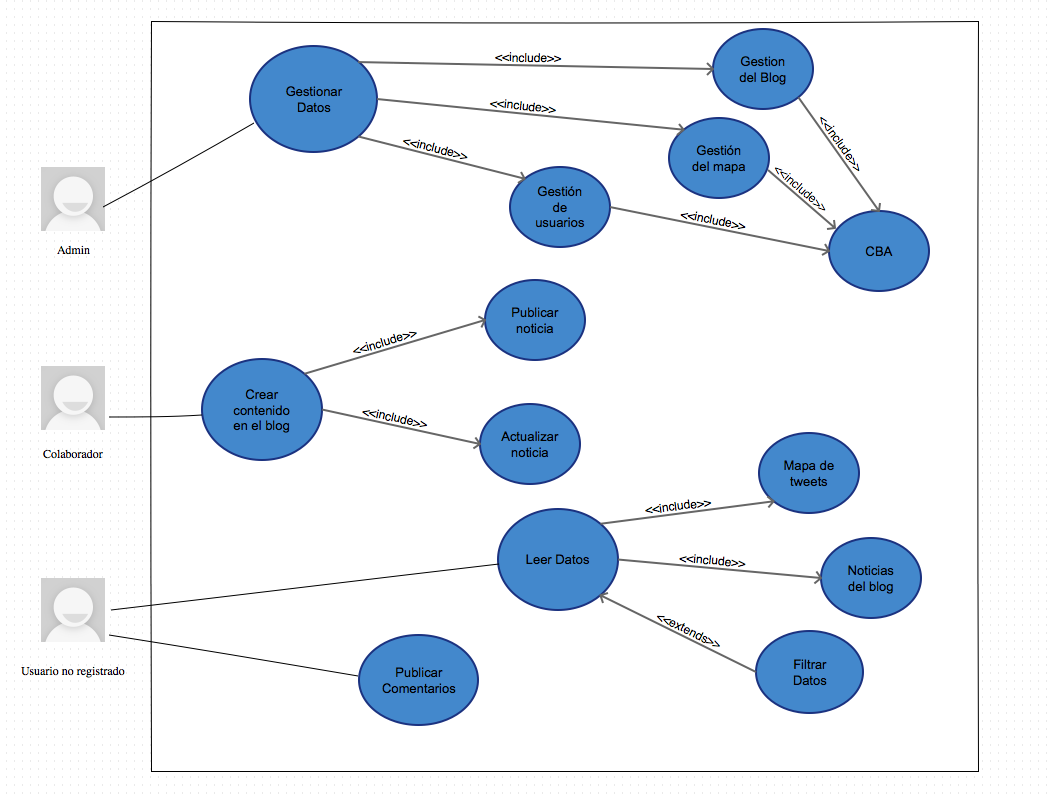
\includegraphics[width=16cm]{imagenes/casos-de-uso.png}
\caption{Casos de uso generales para NjoyCooking}
\label{casos_uso}
\end{center}
\end{figure}
\end{landscape}

Para mostrar las actividades se utilizará una representación mediante casos de uso. Los casos de uso se han segmentado para cada rol de la aplicación. En la figura \ref{casos_uso}  se representan los casos de uso generales para cada rol que se explicarán a continuación:

\vspace{5 mm}

El \textbf{usuario no registrado}. Es el rol por defecto en la aplicación cuando el usuario no tiene ninguna acreditación en la web y carece de permisos. El usuario no registrado podrá solicitar los datos de la aplicación para visualizar el contenido. Por ejemplo podrá solicitar los datos del mapa de tweets o del blog. Tambíen podrá filtrar la información de los datos solicitados, por palabras clave o categorías. Este usuario podrá también publicar comentarios en el blog.

\vspace{5 mm}

El \textbf{colaborador}. Este rol, además de poder realizar las mismas funciones que el usuario no registrado, tiene unos permisos añadidos. Este usuario tiene la función extra de publicar contenido en el blog. Un usuario colaborador, podrá crear noticias que luego aparecerán en el blog. Podrá actualizar las noticias, pero únicamente aquellas que hayan sido creadas por él. No tendrá permisos para borrar contenido del blog.

\vspace{5 mm}

Por último esta el \textbf{administrador}. El rol de administrador, es el de superusuario, ya que posee todos los permisos. El administrador es el encargado de gestionar todo el contenido de la web. Dentro del contenido se encuentran los tres principales modelos de datos. El primer modelo de datos son los \textquote{Tweets}. El administrador se encargará de gestionar la frecuencia con la que se actualiza el mapa de tweets para tener representada la información actualizada. Otra función será modificar la recolección de tweets en base a una palabra clave, que el administrador introducirá manualmente. El siguiente modelo son las noticias, el administrador podrá generar contenido en el blog, creando o borrando cualquier tipo de contenido, tanto propio como de un colaborador. El administrador también podrá moderar los comentarios de las entradas del blog. Finalmente el último modelo de datos serán los usuarios. El administrador gestionará los datos de los usuarios de la aplicación, siendo el encargado tanto de dar de alta a los colaboradores generando un usuario y contraseña como darlos de baja. Toda la gestión del contenido implica crear, borrar o actualizar información de forma que se ha representado mediante el caso de uso CBA.


\section{Diseño de Arquitectura}

\subsection{Arquitectura MVC}

\begin{figure}
\begin{center}
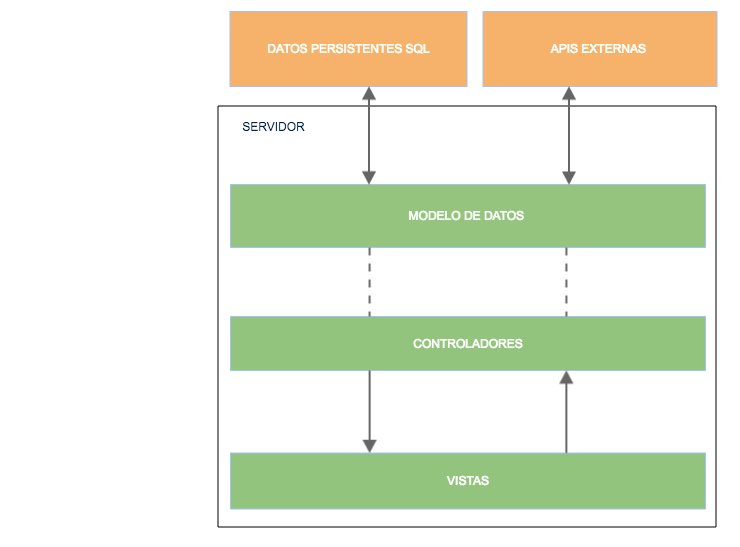
\includegraphics[width=1.0\textwidth]{imagenes/arquitectura.png}
\caption{Arquitectura de la aplicación}
\label{arquitectura}
\end{center}
\end{figure}

La rama de ingenieria del software se preocupa por crear productos robustos y de calidad. Una de las principales soluciones para conseguir esos objetivos es la arquitectura basada en capas, que separa el código en función de sus responsabilidades. Una de las arquitecturas más populares basada en capas para el desarrollo de aplicaciones web, es la arquitectura MVC(Modelo-Vista-Controlador) \cite{mvc}. En la figura \ref{arquitectura} se muestra un esquema de la arquitectura de la aplicación.

\begin{itemize}

\item \textbf{Modelo de datos}. Capa que trabaja con los datos, contiene mecanismos para acceder a la información. A través del modelo accederemos a la base de datos donde,estará la información almacenada. Mediante los modelos también se accederá a los datos de servicios externos que posteriormente se guradarán en la base de datos.

\item \textbf{Controladores}. Responde generalmente a acciones del usuario, e invoca esas peticiones al modelo. También responde al envío de datos a la vista. Los controladores son el núcleo de la aplicación, ya que es aquí donde se procesan todos lo datos antes de ser enviados a la vista. Un controlador consta de varios métodos, cada método se corresponde con una vista y hace uso de las diferentes clases de la capa de modelos de datos.

\item \textbf{Vistas}. Es la capa encargada de presentar la información de nuestra página. Los datos provenientes del controlador se presentan en las vistas para que luego ser renderizada por el navegador.

\end{itemize}

 El flujo de la información en la aplicación sería el siguiente. El usuario accederá a una ruta a través del navegador. Cada ruta de la aplicación se corresponde con una vista, que a su vez esta asociada a un controlador. En el controlador correspondiente se llama a las distintas clases de los modelos. Los modelos conectan con la base de datos, esta le devuelve la información, y es recibida y procesada por los controladores que la envían a la vista para que se visualize en el navegador.


\vspace{5 mm}

Crear una aplicación web basada en la arquitectura MVC nos ofrece ciertas ventajas. Por ejemplo, se puede dividir la lógica del negocio del diseño del sistema, haciendo el proyecto más escalable. Otra ventaja, es la existencia  de muchos frameworks basados en MVC como Laravel o Yii Framework, que permiten facilitar el trabajo de los desarrolladores. La implementación de URLs amigables, el control del uso de la memoria caché o el control de los recursos del servidor son tres de las principales ventajas de usar un framework MVC.


\section{Modelo de Datos}

Como se ha comentado en el apartado anterior, el modelo de datos elegido para almacenar la información es el modelo relacional MySQL. El modelo relacional se fundamenta en el uso de relaciones, estas relaciones se pueden considerar como un conjunto de datos. Para mostrar una forma más visual esas relaciones se conceptualizan en forma de tablas, que estan formadas por registros y campos. En la figura \ref{tablas_bd} se representa mediante un modelo entidad-relacion los conjuntos de datos para la aplicación. Todas las tablas contienen un campo Id que es el identificador de cada tabla(clave primaria) y tienen la clausula de auto-incremento por lo que cada vez que se agregue una fila, MySQL generará otro identificador incrementandolo en 1 valor.


\begin{figure}
\begin{center}
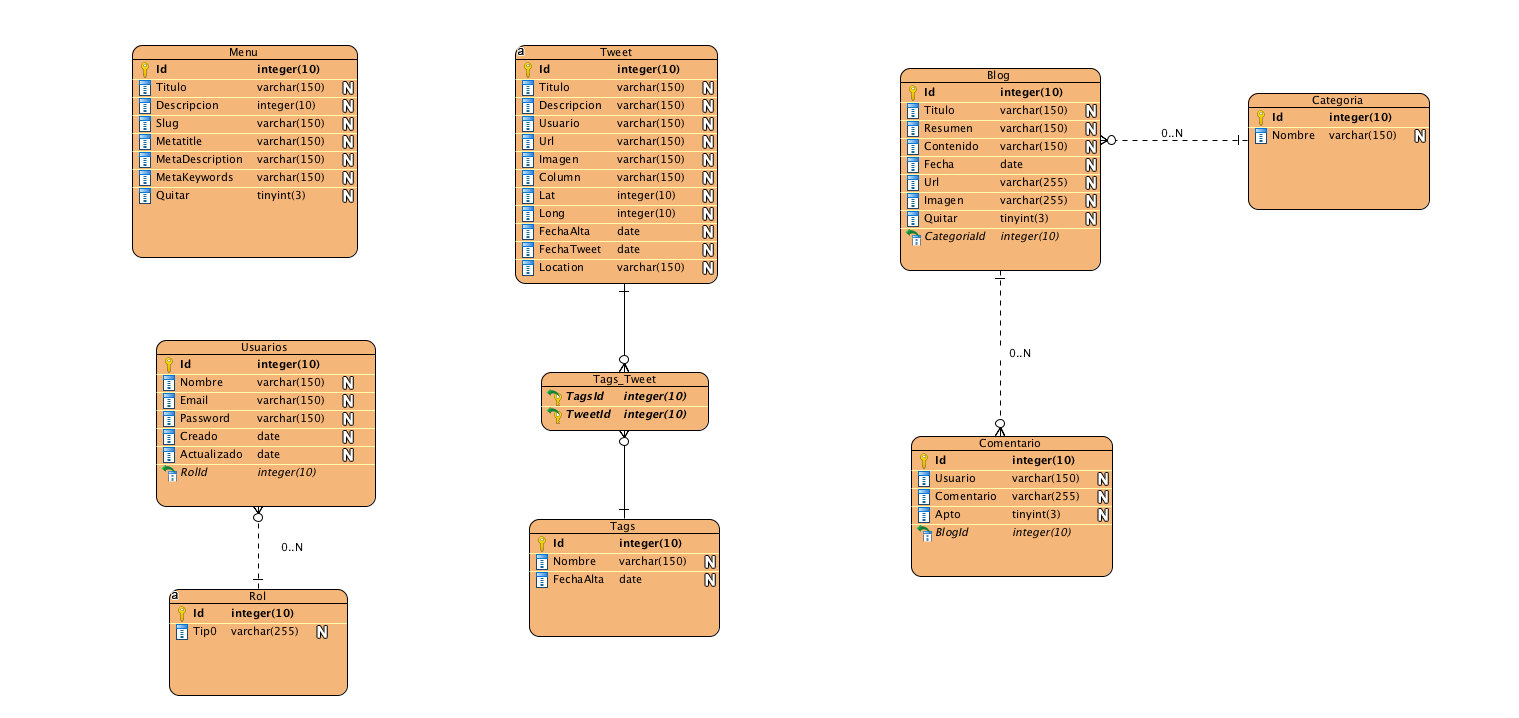
\includegraphics[width=1.0\textwidth]{imagenes/E-R.png}
\caption{Conjunto de tablas}
\label{tablas_bd}
\end{center}
\end{figure}

\begin{figure}
\begin{center}
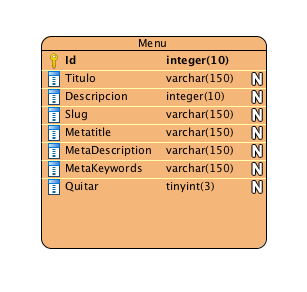
\includegraphics[scale=0.7]{imagenes/menu.png}
\caption{Tabla del menú}
\label{menu_bd}
\end{center}
\end{figure}

\begin{figure}
\begin{center}
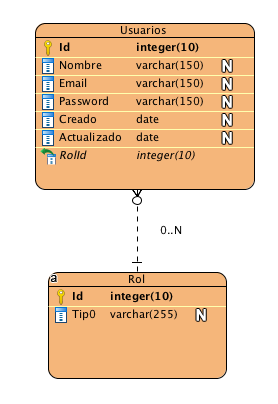
\includegraphics[scale=0.7]{imagenes/Usuarios.png}
\caption{}
\label{users_bd}
\end{center}
\end{figure}

\begin{figure}
\begin{center}
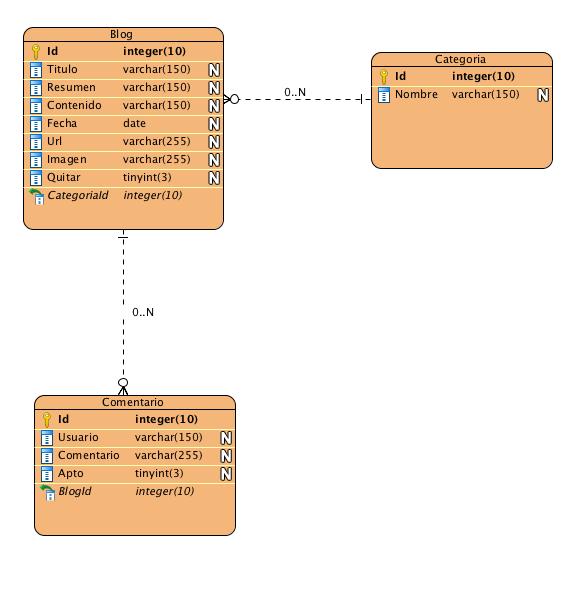
\includegraphics[scale=0.7]{imagenes/blog.png}
\caption{Tablas para el blog}
\label{blog_bd}
\end{center}
\end{figure}

\begin{figure}
\begin{center}
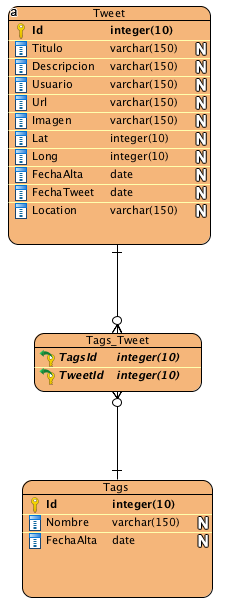
\includegraphics[scale=0.7]{imagenes/map.png}
\caption{Tablas para el mapa}
\label{map_bd}
\end{center}
\end{figure}


\vspace{5 mm}

La primera tabla, y más básica, es la tabla de \textquote{Menus}, en ella encontramos todos los datos correspondientes al menú de navegación de la aplicación,esta tabla esta pensada para que el menú sea más dinamico y se pueda gestionar de forma más fácil sin modificar código. Como se observa en la figura \ref{menu_bd}, la tabla de \textquote{Menus} se compone de los siguientes elementos:

\begin{itemize}

\item \textbf{Título}: Este es el titulo del menú, y el que aparecerá en la web en la navegación.
\item \textbf{Descripcion}: Campo para añadir texto introductorio, acerca de la sección.
\item \textbf{Slug}: El slug corresponde al trozo de la url que aparecerá para esa sección de la web en la aplicación.
\item \textbf{Campos de MetaAtributos}: MetaKeywords,MetaDescription,MetaTitle, los metas para cada sección del menú. Estos campos son importantes para un buen posicionamiento SEO.
\item \textbf{Quitar}: Campo de tipo tinyint, que nos permite dejar de mostrar un elemento del menú sin tener que borrar la fila. Por defecto el campo quitar esta a 0 y por tanto mostrará el elemento, en el caso de no se quiera visualizar, se cambia el valor a 1 y ese elemento ya no se muestra en el menu.

\end{itemize}

\vspace{5 mm}

En la figura \ref{users_bd}, se muestra la tabla de Usuarios y su relación con los Roles de la aplicación. Se pretendía que un usuario tuviera un único rol y que un rol pudiera ser adoptado por muchos usuarios. Para representar esa relación se añade un clave ajena en la tabla usuarios generando una relacion uno a muchos y así permitiendonos cumplir las condiciones dictadas previamente. Para la tabla de Usuarios, se generan los siguientes campos:

\begin{itemize}

\item \textbf{Nombre}. Nombre del usuario, que se muestra en la web.
\item \textbf{Email}. Correo electrónico, del usuario. Tanto este campo como el nombre sirven de login para el usuario.
\item \textbf{Password}. Contraseña del usuario. En la base de datos se guarda un hash de la contraseña para mayor seguridad.
\item \textbf{Creado}. Campo de fecha con la creación del usuario.
\item \textbf{Actualizado}. Campo de fecha con la actualización del usuario.
\item \textbf{RolId}. Clave ajena a la tabla de Rol, contiene el Id del Rol.

\end{itemize}

\vspace{5 mm}

La tabla de Rol únicamente contiene el campo identificador y el tipo que hace referencia al nombre del rol.

\vspace{5 mm}

Para la página del Blog \ref{blog_bd} tenemos el esquema relacional con tres tablas: Blog,Categoría y Comentario. Cada fila de la tabla pertenece a una noticia del blog de la aplicación, cada noticia puede tener uno o más comentarios y ese comentario podrá aparecer solo en una noticia. Por tanto para cumplir esas condiciones se generan dos tablas(Blog y Comentario) con una relación uno a muchos. Las noticias pueden tener categorías, en el caso de la aplicación una noticía puede pertenecer a una categoría o ninguna, por tanto se añade una relación muchos a uno de la tabla Categoría a Blog. Las tuplas para la tabla de Blog son las siguientes:


\begin{itemize}

\item \textbf{Título}. Título de la noticia.
\item \textbf{Resumen}. Campo de texto para mostrar un resumen en el listado de noticias.
\item \textbf{Contenido}. Contenido de la noticia.
\item \textbf{Fecha}. Campo de Fecha con la creación de la noticia.
\item \textbf{Url}. Url amigable que aparece en la ruta de la noticia.
\item \textbf{Imagen}. Campo de texto para la imagen principal de la noticia.
\item \textbf{Quitar}. Campo quitar, para poder dejar de visualizar la noticia sin necesidad de borrarla de la base de datos.
\item \textbf{CategoríaId}. Clave ajena. Id de la categoría a la que pertenece la noticia.

\end{itemize}

\vspace{5 mm}

Tuplas para la tabla de comentarios:

\begin{itemize}

\item \textbf{Usuario}. Usuario que comenta la noticia.
\item \textbf{Comentario}. Campo de texto con el comentario sobre la noticia.
\item \textbf{Apto}. Campo para moderar el comentario y que sea valido para mostrar. Por defecto vale 1, no se muestra, cuando se cambia a cero se valida y se muestra.
\item \textbf{BlogId}. Clave ajena con el Id de la noticia al que pertence el comentario.


\end{itemize}

\vspace{5 mm}

Para el mapa de tweets se generan tres tablas(figura \ref{map_bd}). La principal es la tabla Tweet, donde se almacenan todos los tweets que se van a mostrar en el mapa. Los campos son los siguientes:


\begin{itemize}

\item \textbf{Título}. Título del tweet.
\item \textbf{Descripción}. Campo de texto que contiene el tweet.
\item \textbf{Usuario}. Usuario que ha escrito el tweet
\item \textbf{Url}. Enlace que se encuentra en el tweet y que te lleva a una página externa.
\item \textbf{Imagen}. Imagen del tweet.
\item \textbf{Lat}. Coordenada de latitud en el mapa.
\item \textbf{Long}. Coordenada de longitud en el mapa.
\item \textbf{FechaAlta}. Fecha de registro del tweet.
\item \textbf{FechaTweet}. Fecha de creación del tweet.
\item \textbf{Location}. Campo que guarda una localización.

\end{itemize}


\vspace{5 mm}


Para clasificar el contenido de los tweets, se crea la tabla Tags, que son los distintas clases en las que se pueden clasificar los tweets. Los campos para esta tabla son, el nombre de la etiqueta y la fecha de registro de la misma.

\vspace{5 mm}

Según como esta especificado, un tweet puede tener uno o más tags, y pueden pertenecer varios tweets a un tag. Por tanto es una relación muchos a muchos, para cumplir esta relación se crea una tabla adicional(Tag\_Tweets), que contiene los identificadores(es decir las claves primarias) de las dos tablas relacionadas(Tweet y Tag).

\chapter{Implementación}

\section{Software}

Para diseñar una interfaz de usuario real, en la que poder basarme para luego representarla mediante HTML y CSS, se utilizan diversos programas de diseño web.

\begin{itemize}

\item \textbf{Sketch}: Sketch es una aplicación de diseño vectorial, que te permite diseñar interfaces para aplicaciones móviles o web de una manera sencilla y con una gran potencia.
\item \textbf{Illustrator}: Esta herramienta de adobe tan famosa, te permite el diseño de logotipos de forma vectorial,
\item \textbf{Spectrum}: Programa sencillo que te permite crear paletas de colores, de forma que puedas seleccionar colores complementarios o de gama monocromática y utilizarlos para la interfaz de la aplicación.

\end{itemize}

\section{Tecnologías}

Para la realización de la aplicación web, se ha llevado a cabo un análisis de las tecnologías disponibles, y se han seleccionado las que mejor se adaptaban a las necesidades del proyecto.

\subsection{Front-End(Cliente)}

Las dos principales e indispensables tecnologías que se usan para la parte del cliente son el lenguaje de etiquetas HTML5 y las hojas de etilos CSS3. Estas son dos de las tecnologías fundamentales en las que se basa el desarrollo web.

 \vspace{5 mm}

 Con la finalidad de conseguir una apariencia cuidada e intuitiva del sitio web, sin la necesidad de crear las hojas de estilos propias, se planteó la idea de usar el framework Bootstrap. Finalmente debido al objetivo de personalizar al máximo la apariencia de la web, se descartó Bootstra y se optó por añadir clases propias mediante css.

\vspace{5 mm}

Para maquetar el sitio web con CSS3 de forma más rápida y refactorizable se utiliza \textbf{Sass}. Sass es un lenguaje de preprocesado de CSS, que permite escribir CSS de forma más cómoda, posibilitando declarar variables,mixins, herencia de clases, etc. Hay diversas formas de utilizar Sass en tu proyecto. Mediante un programa como Prepros, mediante un automatizador de tareas como Grunt, o mediante un terminal con los comandos de Sass. Para el proyecto yo he optado usar el terminal para ejecutar Sass, ya que su ejecución es mucho más ligera y consume menos RAM que con programas como Prepros. Para que empezar a usar Sass en el proyecto, dentro de nuestra carpeta padre donde se encuentre el css, se crea una carpeta sass donde se incluirán todos los ficheros .scss. Con el terminal situado en la carpeta padre escribimos sass --watch sass(nombre de la carpeta donde se encuentran los ficheros .scss). Al compilarlo, generará un fichero style.css que será la hoja de estilo a usar.

\vspace{5 mm}

Para añadir el dinamismo a la web, se ha optado por utilizar un framework de Javascript como \textbf{JQuery} que permite simplificar la manera de interactuar con los documentos HTML, manipular el DOM, desarrollar animaciones y agregar peticiones AJAX. Además de que JQuery es software libre.

\vspace{5 mm}

Como última tecnología Front-End se utiliza la API de Google Maps, indispensable para el sitio web ya que la principal proposición de valor de la aplicación es la geolocalización de recetas, y para su representación necesitamos la API de Google.


\subsection{Back-End(Servidor)}

Después de barajar diversos lenguajes para desarrollar el back-end de la aplicación, finalmente se eleigió PHP. Además de ser el lenguaje más utlizado para el desarrollo web, es uno de los lenguajes más potentes y flexibles, pudiendo ser utilizado en la mayoría de los servidores web y sistemas operativos. Además PHP esta publicado bajo licencia de software libre, por lo que no supone ningun coste.


\vspace{5 mm}

Para montar la arquitectura MVC en la aplicación, se utiliza el framwework Laravel. Laravel agiliza el desarrollo de las aplicaciones web, permitiendo multitud de funcionalidades. Con este framework, desarrollado de forma elegante y simple se evita la creación de código espagueti, faciltando su refactorización y/o su modificación. Algunas de las carácterísticas de Laravel: 


\begin{itemize}

\item \textbf{Plantillas}: Laravel utiliza platillas Blade. Blade permite tener un sitema de vistas modular de forma que se tenga que repetir la menor cantidad de código. Para ello se genera una plantilla base o layout, que es donde se representa la estructura de la web y se volcará el contenido para cada página. Mediante la directiva include(nombre\_template), se podrá incluir una vista parcial de contenido HTML, esta directiva se utiliza para contenido que no cambia por ejemplo para incluir la cabecera o el footer de la aplicación. Luego mediante la sentencia yield(nombre\_template) permitiremos crear una futura sección en el HTML que se definirá en las vistas que son heredadas de este template. Mediante la sentencia extends(nombre\_template) le diremos a Laravel que vistas se van a usar como futuras secciones. Con estas sentencias se conseguirá volcar el contenido especifíco para cada página de la web duplicando el menor numero de codigo HTML y de forma más modular.

\item \textbf{ORM}: Es una implementación de registro activo para trabajar con la base de datos de forma que cada tabla de la base de datos tiene un Modelo correspondiente asociado con el mismo nombre. Esta implementación te permite también métodos predefinidos para llamar a la base de datos como save(),create(),get(),find().

\item \textbf{Caché}: Laravel, cuenta con un robusto sistema de caché, el cual se puede ajustar, para que se produzca una carga rápida de la web y generar una mejor experiencia al usuario.

\item \textbf{MiddleWare}: Usa HTTP Middleware, que proporcionan un correcto mecanismo para filtrar las peticiones en la aplicación. Un ejemplo de middleware que incluye laravel, es el usado para verificar si el usuario esta autenticado en la aplicación.

\end{itemize}

\vspace{5 mm}

Para la base de datos, se utiliza el sistema de gestión relacional MySQL, ya que es uno de los sistemas más utilizados y con mayor documentación para el desarrollo web. Además, de la perfecta integración con Laravel.

\subsection{Estructura de la aplicación}

Para comenzar a desarrollar el proyecto, primero se debe instalar Laravel. Para ello se utiliza un manejador de dependencias como composer que nos permite instalar los paquetes y librerías de forma automática sin la necesidad de hacerlo de forma manual. Mediante nuestro terminal escribimos el siguiente código para instalar composer en el ordenador: curl -sS https://getcomposer.org/installer | php. Una vez instalado, para generar un proyecto con laravel escribimos en el terminal el siguiente comando: composer create-project laravel/laravel nombre-proyecto.

\vspace{5 mm}

\begin{figure}
\begin{center}
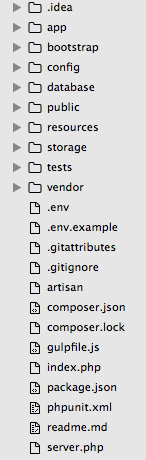
\includegraphics[width=1.0\textwidth]{imagenes/estructura-laravel.png}
\caption{Proyecto de Laravel}
\label{laravel}
\end{center}
\end{figure}

Si vamos a la carpeta raiz con la que creamos el proyecto se observa que dentro composer ha generado una estructura de directorios(figura \ref{laravel}) que es como organiza Laravel el código de la aplicación. A continuación se detallan brevemente cada una de ellas:


\begin{itemize}

\item \textbf{app}: el directorio app es donde se encontrará la mayor parte del código personal del back-end de la aplicación. Desde los modelos de datos de la aplicación, hasta los controladores pasando por el middleware.

\item \textbf{config}: aqui se encuentran los ficheros de configuración de Laravel y de la aplicación. Por ejemplo en el fichero app.php se especifican parametros tales como la zona horaria y el idioma de la aplicación. También se definen los providers, que son cada uno de los objetos o instancias que se cargarán en el proyecto. 

\item \textbf{database}: aquí se encuentran todos los ficheros relacionados con la base de datos de la aplicación. Dentro encontramos tres subdirectorios:

- factories: aquí se incluyen los ficheros que generan automaticamente nuevos datos en tu base de datos para testear la aplicación, sin necesidad de generarlos manualmente.

- migrations: las migraciones son un tipo de control de versiones para la base de datos. A través de estos ficheros se puede modificar la base de datos.

- seeds: permiten poblar la base de datos con datos de prueba. Los seeds pueden utilizar factories para poblar la base de datos o introudcirlos manualmente.

\item \textbf{public}: en este directorio se encuentran los directorios con ficheros estáticos como son las hojas de estilo(css), los ficheros javascript(js) y las imágenes(images).

\item \textbf{resources}: en resource encontramos subdirectorios donde se encuentran las vistas  en formato blade.php de la aplicación(views) y los archivos de idiomas de la aplicación, para poder pasar de un idioma a otro en la aplicación(lang).

\item \textbf{storage}: se encuentran varios subdirectorios que contiene el cache de la aplicación, sesiones, etc.

\item \textbf{vendor}: este directorio contiene todo el core de Laravel y los componentes instalados.

\end{itemize}

\begin{figure}
\begin{center}
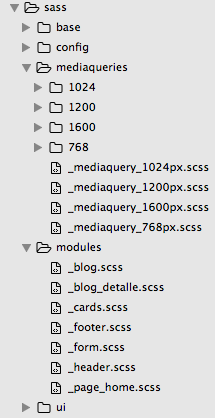
\includegraphics[width=1.0\textwidth]{imagenes/estructura-sass.png}
\caption{Estructura Sass}
\label{sass}
\end{center}
\end{figure}

\textbf{Estructura Sass} 

Como se comenta previamente, se utiliza Sass para maquetar la web. Este lenguaje de preprocesado de Css te permite organizar el ccs y hacerlo más modular de forma que puedes generar varios ficheros .scss y compilarlos en un único fichero css que es el que se utilizará en la aplicación. Para ello uso una carpeta sass que se incluye en la carpeta public del proyecto donde incluyo todos los directorios con los ficheros sass. Una de las formas de refactorizar más el código Sass, es generar un fichero .scss para cada página web de la aplicación de modo que en futuros cambios resulte todavía más sencillo modificar el estilo. Como se observa en la figura \ref{sass} la estructura sass es al siguiente:


\begin{itemize}

\item \textbf{base}: en el directorio base se encuentran los ficheros scss con los elementos más básicos de la aplicación. Las tipografías usadas, los formatos de texto de los encabezados y párrafos, etc.

\item \textbf{config}: en este directorio encontramos los siguientes ficheros.

- variables: scss donde se declaran las variables que se usan en las hojas de estilo tales como colores de la aplicación, las fuentes usadas.

- functions: aquí se encuentran los mixins de sass que se pueden utilizar. Los mixins no son más que funciones que te permiten reutilizar estilos.

- animations: en este directorio se incluyen los ficheros scss con animaciones hechas con css incluidas en la aplicación.

\item \textbf{ui}: en el directorio ui(user interface) se incluyen los ficheros scss que modifiquen las propiedades css de elementos de la interfaz gráfica de la aplicación como botones,formularios, etc.

\item \textbf{modules}: debido a que la aplicación esta basada en la filosofía mobile first en esta carpeta se incluyen todos lo ficheros scss de las páginas de la aplicación en resolución móvil(de 0 a 768px de resolución de pantalla).

\item \textbf{mediaqueries}: en esta carpeta se incluyen los ficheros scss para las resoluciones de tablet y ordenador de escritorio. Para esta resolución se han marcado las resolución de 768px a 1024px(tablet) y para escritorio las resoluciones de 1024px a 1600px y mayores de 1600px. Para cada resolución habrá un subdirectorio con el nombre de la resolución donde se incluirán sus ficheros scss correspondientes.


\end{itemize}

\vspace{5 mm}

\section{Sprints}

Una instalado el framework Laravel y comprendida su estructura se procede a desarrollar la aplicación. Para realizar el proyecto, como se especifica previamente se utiliza la metodología Scrum. El proyecto se divide en los siguientes sprints:


\subsection{Diseño y maquetación de la interfaz}

\begin{figure}
\begin{center}
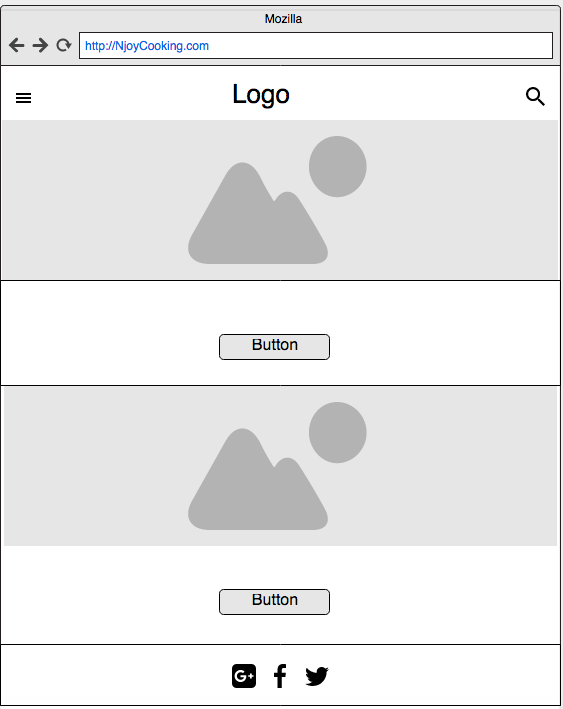
\includegraphics[width=1.0\textwidth]{imagenes/landing.png}
\caption{Landing}
\label{landing}
\end{center}
\end{figure}

\begin{figure}
\begin{center}
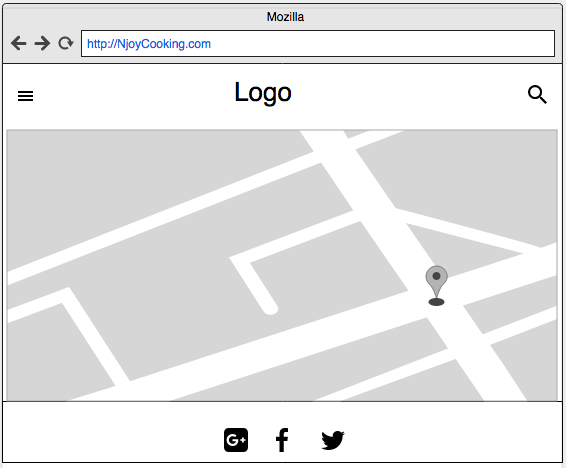
\includegraphics[width=1.0\textwidth]{imagenes/mapa.png}
\caption{Mapa}
\label{mapa}
\end{center}
\end{figure}

\begin{figure}
\begin{center}
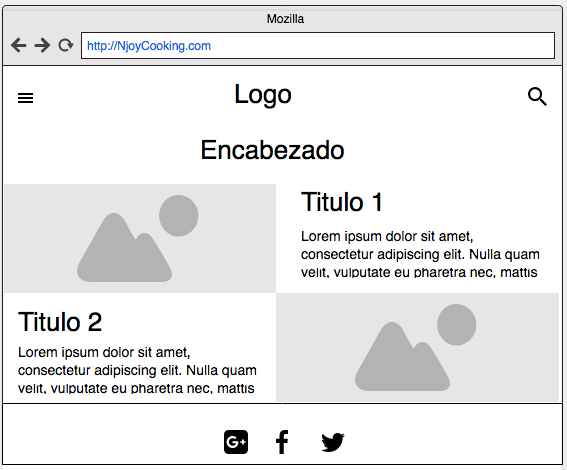
\includegraphics[width=1.0\textwidth]{imagenes/listado-blog.png}
\caption{Listado de noticias}
\label{listado-blog}
\end{center}
\end{figure}

\begin{figure}
\begin{center}
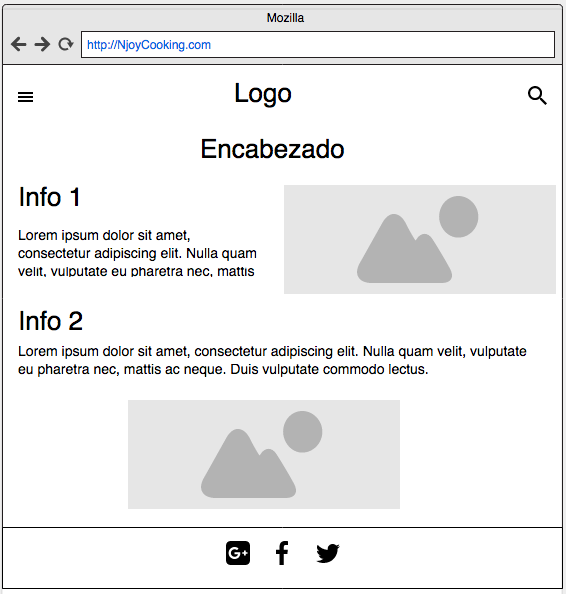
\includegraphics[width=1.0\textwidth]{imagenes/detalle-blog.png}
\caption{Detalle de noticia}
\label{detalle-blog}
\end{center}
\end{figure}

Inicialmente se llevan a cabo unos bocetos de la web mediante mockups para saber como se va a organizar el contenido de la aplicación.

\vspace{5 mm}

Cualquier empresa que se encuentre en el mundo de las aplicaciones web sabe que una landing, es la mejor forma de promocionar el producto o marca que se quiere dara conocer. Por eso a la página inicial donde el usuario accederá será una landing donde se mostrará información acerca de los servicios que ofrece la web.

\vspace{5 mm}

Como se observa en el boceto(figura \ref{landing}) la landing tiene un diseño sencillo y usable. En esta página se mostrarán una series de secciones informativas acerca de los contenidos disponibles de la web y otras informaciones relevantes. Las secciones irán acompañadas de una imagen de fondo, un texto informativo y un botón que te dirige a la página correspondiente.

\vspace{5 mm}

La cabecera de la landing, que será común a todas las páginas de la web, tendrá un diseño responsive para todas las resoluciones. El menú será desplegable de forma que al pulsar sobre el icono de  la hamburguesa se verán todas las secciones por las que se podrá navegar por la web. Este menú mobile se ha aplicado para la resolución de escritorio ya que favorecía a conseguir una mayor limpieza de la interfaz,no empeoraba su usabilidad y le daba un aspecto más minimalista. Además de este menú en la cabecera encontraremos el logo de la web y un buscador global de la web. Esta cabecerá siempre estará fija para favorecer la usabilidad al usuario.

\vspace{5 mm}

Por último, el footer o pie de página, otro elemento común a todas las páginas. En esta sección se mostrarán las distintas redes sociales de la empresa, los textos legales(copyright,privacidad) y el logo de la web.


\vspace{5 mm}

La siguiente página, es la del mapa (figura \ref{mapa}). En esta página se mostraban un mapa con los marcadores de las recetas geoposiconadas. El diseño de esta página es muy sencillo ya que además de los elementos comunes de cabecera y pie, en el contenido se muestra un elemento con el mapa que va a mostrar la información.

\vspace{5 mm}

La próxima sección, es la sección del blog que se compone de dos páginas: el listado de noticias y el detalle de noticia. En el listado de noticias(figura \ref{listado-blog}), el primer elemento que se mostrará será un encabezado con una foto y descripción de la sección del blog. A continuación se mostrarán un listado con las diferentes noticias del blog y en cada una se mostrará un foto, un título y un resumen. Para esta sección la disposición de los elementos de la notícia en movil cambiará colocando los elementos en una sola columna en vez de dos como se muestran en tablet y pc.

\vspace{5 mm}

En el detalle de la receta(figura \ref{detalle-blog}) se muestra toda la información asociada a esa noticia.




%input{capitulos/resultados}
%input{capitulos/conclusiones}

%%\nocite{*} %incluye TODOS los documentos de la base de datos bibliográfica sean o no citados en el texto
%\bibliography{bibliografia/bibliografia}\addcontentsline{toc}{chapter}{Bibliografía} %sustituir bibliografía con el nombre del fichero bibtex con la bibliografía
%\bibliographystyle{apalike}
%
\appendix
%\chapter{Anexo I}
Aquí vendría en anexo I 
%\input{glosario/entradas_glosario}
% \addcontentsline{toc}{chapter}{Glosario} %si se usa glosario hay que añadirlo al índice
% \printglossary %muestra el glosario

\end{document}
